\documentclass[a4paper, 12pt]{book}

% úprava rozměrů strany a okrajů
\usepackage[top=1.5cm, left=1.5cm, right=1.5cm, bottom=1.5cm]{geometry}

% nastav kódování na vstupu
\usepackage[utf8]{inputenc}

% nastav jazyk
\usepackage[czech]{babel}

% zrušení číslování
\pagestyle{empty}

% zrušení odsazování odstavců
\def\everypar{\parindent=0cm}

% neproporcionální písmo
\renewcommand*\familydefault{\ttdefault}

% jednotný formát názvů písní a interpretů
\newcommand{\song}[2]{%
\section*{\Huge\expandafter\MakeUppercase\expandafter{#1}}
\vspace{-1em}\emph{#2}\newline
}

\usepackage{pdfpages}

% refren
\newenvironment{chorustext}{\begin{em}}{\end{em}}

\newcommand{\chorus}{\textregistered}

\newcommand{\7}{\textsuperscript{7}}
\newcommand{\9}{\textsuperscript{9}}

\begin{document}

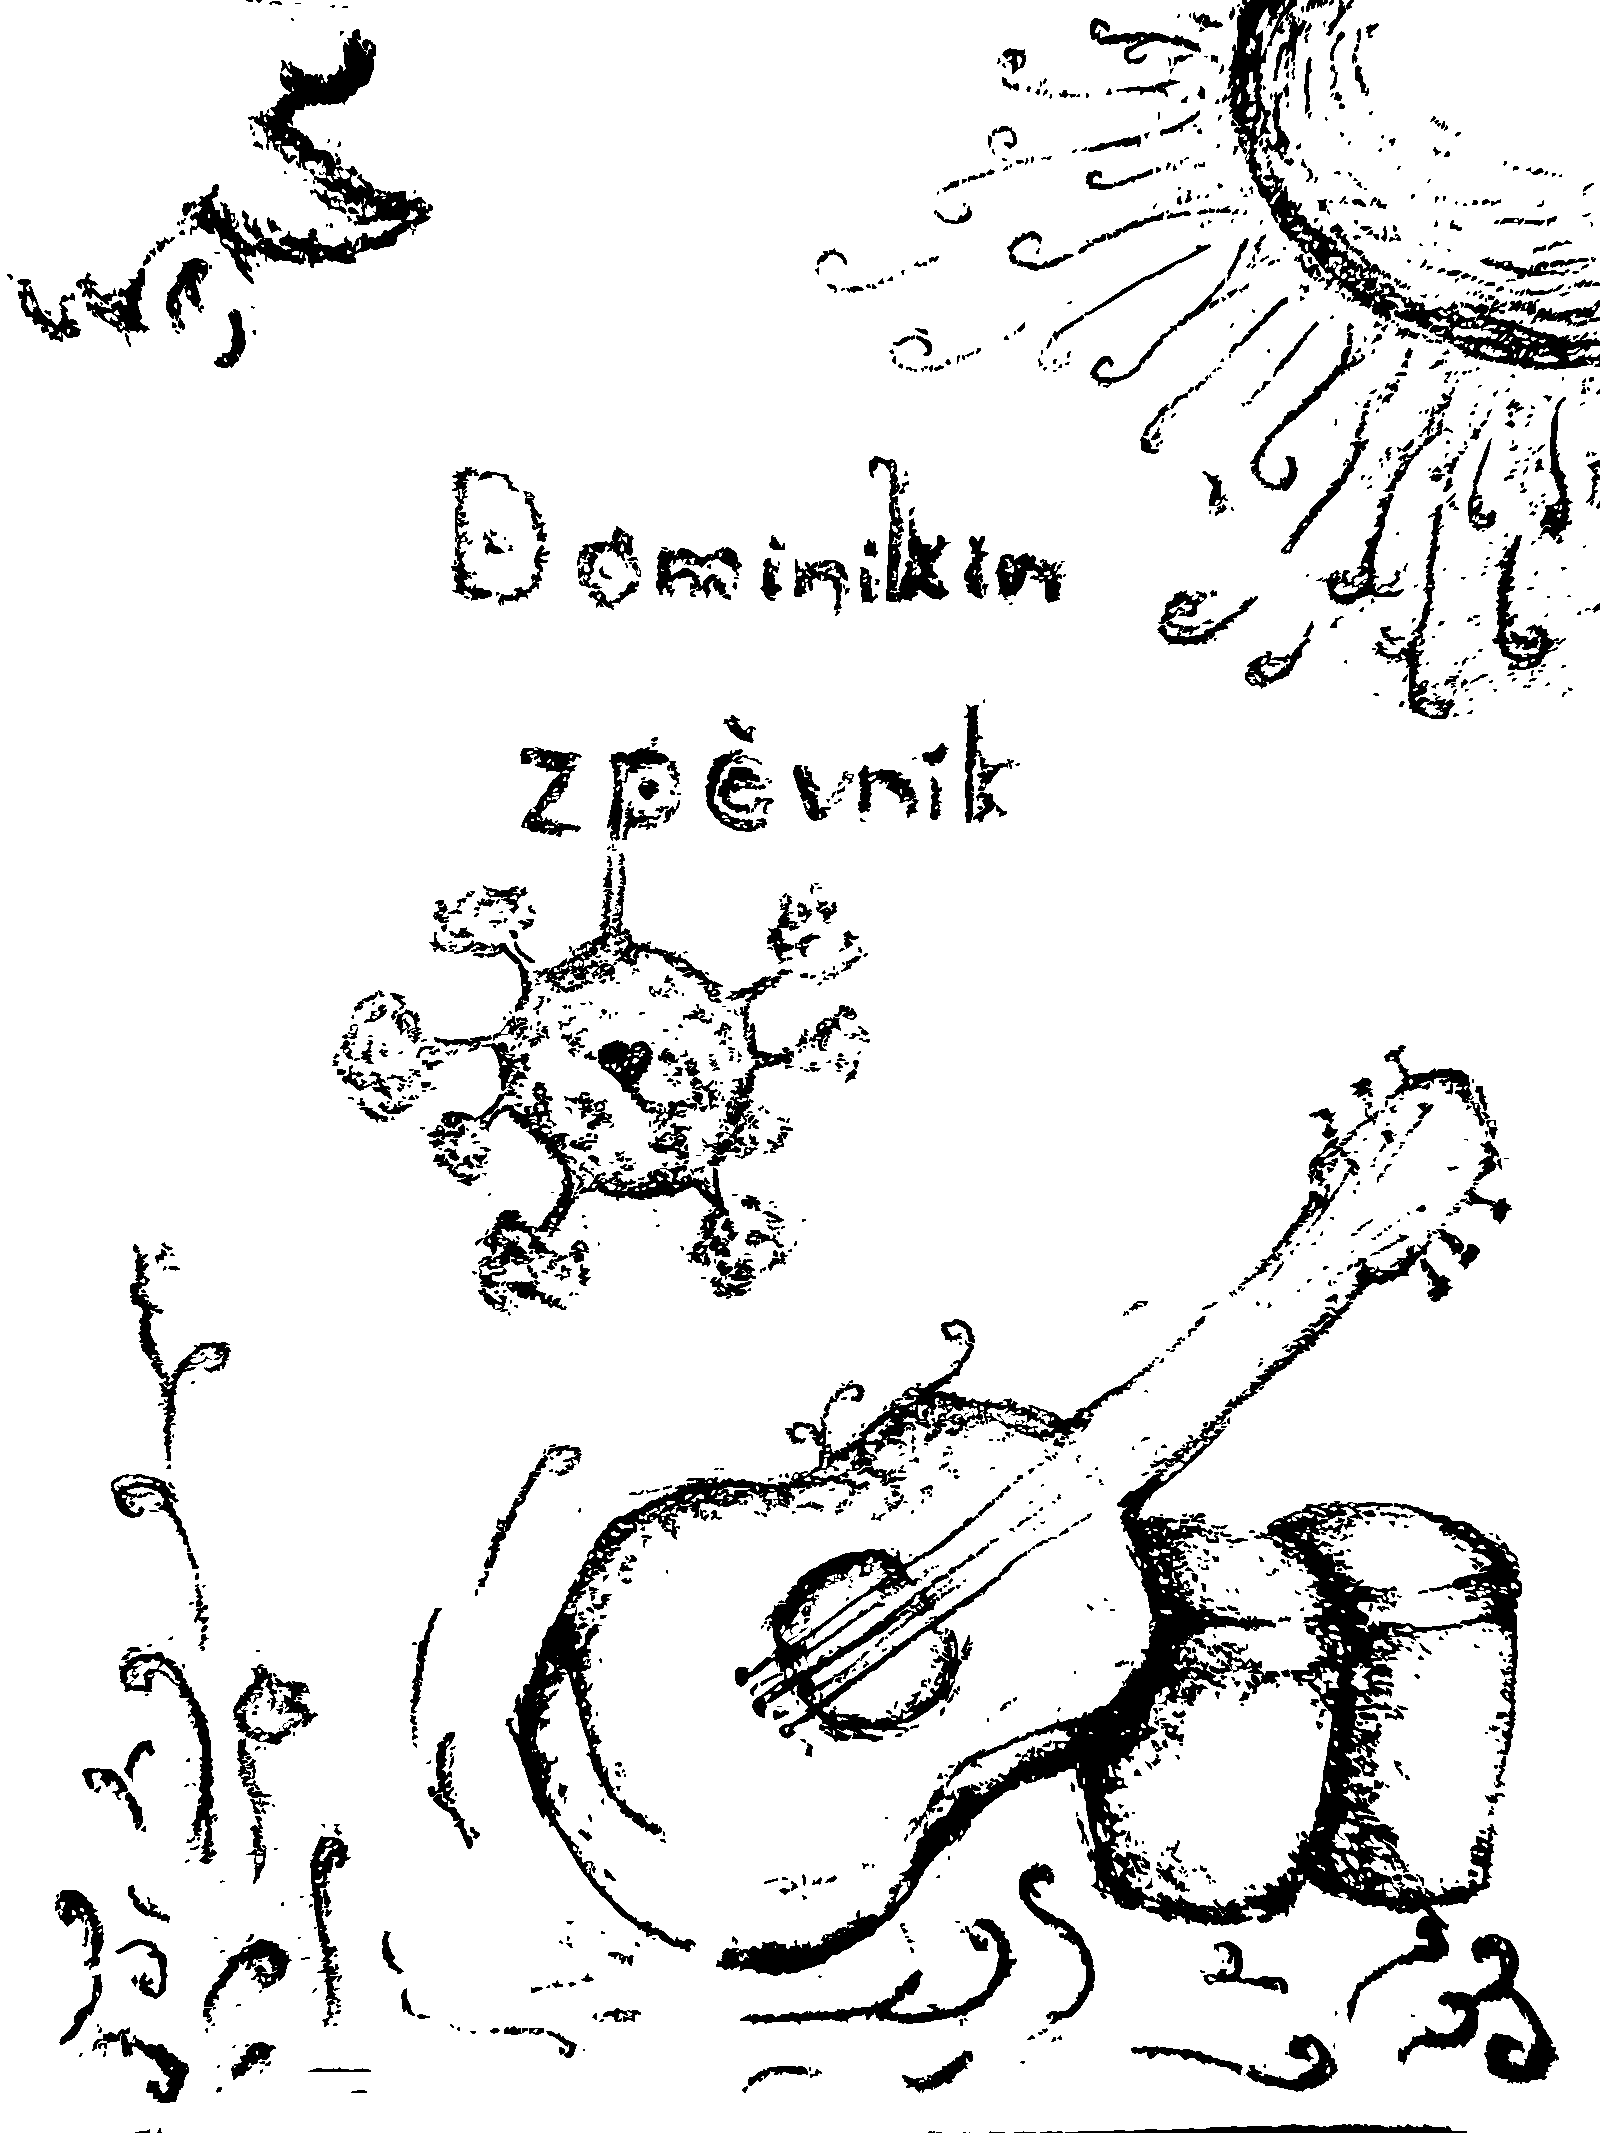
\includepdf{titulka.pdf}

\begin{LARGE}
    \section*{\Huge OBSAH}
\end{LARGE}

\begin{multicols}{2}

\subsection*{A}
All you need is love (The Beatles)

Amavi te puella

Amerika (Lucie)

Anděl (Karel Kryl)

Atentát (Kryštof)

\subsection*{B}
Bim bam

Blowin in the wind (Bob Dylan)

Bonsoir mademoiselle Pari (Petr Muk)

Buď vôľa tvoja (Krížik)

Buráky

\subsection*{C}
Cesta (Kryštof \& Tomáš Klus)

Counting stars (OneRepublic)

Cups (Anna Kendrick)

Cysta (Ruda z Ostravy)

\subsection*{Č}
Čarodějnice z Amesbury (Asonance)

Černý muž

Čert ví kdy kotvy zvednem (Waldemar Matuška)

Červená řeka

\subsection*{D}
Darmoděj (Jaromír Nohavica)

Den je krásný (\emph{Starci na chmelu})

Dobrý Václav král

Drunken sailor (Irish Rovers)

Dům u vycházejícího slunce

\subsection*{E}
Every breath you take (The Police)

\subsection*{F}
Falling slowly (Glen Hansard \& Markéta Irglová)

\subsection*{G}
Gastrosexuál (Wohnout)

Good king Wenceslas

\subsection*{H}
Happy ending (Mika)

Hey Jude (The Beatles)

Hrobař (Premiér)

Hříšná těla křídla motýlí (Aneta Langerová)

Hvězdičko blýskavá (Petr Novák)

Hvězdy se mění (Jan Kalousek)

\subsection*{CH}
Christmas is all around (\emph{Láska nebeská)}

\subsection*{I}
Irský hody (Kabát)

\subsection*{J}
Jablíčko (\emph{Cikáni jdou do nebe})

Jaro (Fešáci)

\subsection*{K}
Když náš táta hrál (Greenhorns)

Komáři se ženili

Kozel (Jaromír Nohavica)

\subsection*{L}
L.A.G. song (Horkýže Slíže)

Lachtani (Jaromír Nohavica)

Lokomotiva (Poletíme?)

\subsection*{N}
Na na na (No Name \& Chinaski)

Nebude to ľahké (Richard Müller)

\subsection*{O}
Okno mé lásky (Olympic)

\subsection*{P}
Pátá (\emph{Rebelové})

Po schodoch (Richard Müller)

Pocit (Divokej Bill)

\subsection*{R}
Raci v práci (Kabát)

Ráda se miluje (Karel Plíhal)

Radioactive (Imagine Dragons)

\subsection*{S}
Starosta (No Name)

Stonka (Kristina)

\subsection*{Š}
Šneček

\end{multicols}


\newpage


\subsection*{T}
Touha (Daniel Landa)

Tři citrónky

Tučňák z Antarktidy (DRON \emph{K-SCUK 2016})

\subsection*{V}
V blbým věku (Xindl X)

Věčnost (No Name)

Vezmi ma (Heartbeat)

\subsection*{Z}
Zafúkané (Fleret)

\subsection*{Ž}
Ženy (Kryštof)

Žily (No Name)

\newpage


\song{Amerika}{Lucie}

G~~~~~~~~~D~~~~~~~~~~~~Ami~~~

Nandej mi do hlavy tvý brouky

~~~~~~~~~~~~~~~~~~~~~G~~

A Bůh nám seber beznaděj

~~~~~~~~~~~~~D~~~~~~~~~~~~~~Ami~~

V duši zbylo světlo z jedný holky

~~~~~~~~~~~~~~~~~~~~~~G~

Tak mi teď za to vynadej

~~~~~~~D~~~~~~~~~~Ami~~

Zima a promarněný touhy

~~~~~~~~~~~~~~~~~~~~~~G~~~

Do vrásek stromů padá déšť

~~~~~~~~~~~~~D~~~~~~~~~~Ami~~~

Zbejvaj roky asi ne moc dlouhý

~~~~~~~~~~~~~~~~~~C~~~~~~D~~~~~G~

Do vlasů mi zabroukej pá pa pá pá

\bigskip

\begin{chorustext}

~~~~G~~~~~~~~Emi~~~~~~~~~~G~~~~~~~~~~~~Emi~~~~~~~~~~G~~

\chorus:~pá pá pa pá, pá pa pá pá, pá pa pá pá, pá pa pá pá

\end{chorustext}

\bigskip

G~~~~~~~~~D~~~~~~~~~~~Ami~

Tvoje oči jenom žhavý tóny

~~~~~~~~~~~~~~~~~G~

Dotek slunce zapadá

~~~~~~~~~~~~D~~~~~~~~~~Ami~~

Horkej vítr rozezní mý zvony

~~~~~~~~~~~~~~~~~~C~~~~~D~~~~~G~

Do vlasů ti zabrouká pá pa pá pá

\bigskip

\chorus \chorus

\bigskip

G~~~~~~~~~D~~~~~~~~~~~~~~~Ami~~

Na obloze křídla tažnejch ptáků

~~~~~~~~~~~~~~~~~~~~~~~~~G~~

Tak už na svý bráchy zavolej

~~~~~~~~~~~~D~~~~~~~~~~~~Ami~~

Na tváře ti padaj slzy z mraků

~~~~~~~~~~~~~~~~~~~~~G~~

A Bůh nám sebral beznaděj

~~~~~~~~~~~~~~~D~~~~~~~~~~~~~~Ami~~

A v duši zbylo světlo z jedný holky

~~~~~~~~~~~~~~~~~~~~~~G~~~

Do vrásek stromů padá déšť

~~~~~~~~~~~~~D~~~~~~~~Ami~

Poslední dny hodiny a roky

~~~~~~~~~~~~~~~~~~C~~~~~D~~~~~G~

Do vlasů ti zabrouká pá pa pá pá

\bigskip

\chorus

\song{Bedna od whisky}{}
Ami~~~~~~~~~~C~~~~~~~~Ami~~~~~~~~~~~~~E\7

Dneska už mi fóry ňák nejdou přes pysky,

Ami~~~~~~~~~~~~~~C~~~~~~~~~~~Ami~~~E\7~~~~~~Ami

stojím s dlouhou kravatou na bedně vod whisky,

Ami~~~~~~~~~~~~~~C~~~~~~~~Ami~~~~~~~~~~E\7

stojím s dlouhým vobojkem jak stájovej pinč,

Ami~~~~~~~~~~~~C~~~~~~~~~Ami~~~~~E\7~~~~~Ami

tu kravatu, co nosím, mi navlík' soudce Lynč.

\bigskip

\begin{chorustext}

~~~~A~~~~~~~~~~~~~~~D~~~~~~~~~E~~~~~~~~~~~~A

\chorus: Tak kopni do tý bedny, ať panstvo nečeká,

~~~~~~~~~~~~~~~~~~~D~~~~~~~~~E~~~~~~~~~~A

jsou dlouhý schody do nebe a štreka daleká

~~~~~~~~~~~~~D~~~~~~~~E~~~~~~~~~~~~A

do nebeskýho baru, já sucho v krku mám,

~~~~~~~~~~~~~~~~D~~~~~~~~~~E~~~~~~~~~~A

tak kopni do tý bedny, ať na cestu se dám.
\end{chorustext}

\bigskip

Ami~~~~~~~~~~~~~C~~~~~~~~~Ami~~~~~~~~E\7

Mít tak všechny bedny vod whisky vypitý,

Ami~~~~~~~~~~~C~~~~~~~~~~~~Ami~~~E\7~~Ami

postavil bych malej dům na louce ukrytý,

Ami~~~~~~~~~~~C~~~~~~~~~~~Ami~~~~~~~~~~~~E\7

postavil bych malej dům a z vokna koukal ven

Ami~~~~~~~~~~~~~~~~~C~~~~~~~~~~Ami~~~~~~E\7~~~~~Ami

a chlastal bych tam s Billem a chlastal by tam Ben.

\bigskip

\chorus

\bigskip

Ami~~~~~~~~~~~~~~~C~~~~~~Ami~~~~~~~~~~E\7

Když jsem štípnul koně a ujel jen pár mil,

Ami~~~~~~~~~~~C~~~~~~~~~~Ami~~~~E\7~~Ami

nechtěl běžet dokavád se whisky nenapil,

Ami~~~~~~~C~~~~~~~~~~Ami~~~~~~~~E\7

zatracená smůla zlá, zatracenej pech,

Ami~~~~~~~~~~~C~~~~~~~~~~Ami~E\7~~~Ami

když kůň cucá whisku jak u potoka mech.

\bigskip

\chorus

\bigskip

Ami~~~~~~~~~~~C~~~~~~~~~~Ami~~~~~~~~~~~E\7

Kdyby jsi se, hochu, jen pořád nechtěl rvát,

Ami~~~~~~~~~C~~~~~~~~~Ami~~~E\7~~~~Ami

nemusel jsi dneska na týhle bedně stát,

Ami~~~~~~~~~~~~~~C~~~~~~~~Ami~~~~~~~~~~E\7

moh' jsi někde v suchu tu svoji whisky pít,

Ami~~~~~~~~~C~~~~~~~~~Ami~~E\7~~~Ami

nemusel jsi dneska na krku laso mít.

\bigskip

\chorus

\bigskip
\newpage %%%

Ami~~~~~~~~~~~~~C~~~~~~~~~~Ami~~~~~~~E\7

Až kopneš do tý bedny, jak se to dělává,

Ami~~~~~~~~C~~~~~~~~~~~Ami~~~E\7~~Ami

do krku mi vostane jen dírka mrňavá,

Ami~~~~~~~~~C~~~~~~~~Ami~~~~~~~~~~~E\7

jenom dírka mrňavá a k smrti jenom krok,

Ami~~~~~~~~~~~C~~~~~~~Ami~~~~E\7~~Ami

má to smutnej konec a whisky ani lok.

\bigskip

\chorus

\song{Colorado}{Kabát}

~~~~~G~~~~~~~~~~~~~~~~~~~~~~~~~~C

Táta vždycky říkal: Hochu žádný strachy,

~~~~~~~~~~~~~G~~~~~~~~~~~~~~~~~~~~~~D

jseš cowboy, v Coloradu můžeš krávy pást.

~~~~~~~~~G~~~~~~~~~~~~~~~~~~~~~~~~~~C

Já radši utratil jsem psa a všechny prachy,

~~~~~~~~~G~~~~~~~~~D~~~~~~~~~~~~~~G
         
do srdce Evropy já vodjel v klidu krást.

\bigskip

~~~~~~~~G~~~~~~~~~~~~~~~~~~~~~C

Narvaný kapsy prsteny, řetězy zlatý,

~~~~~~~~~~G~~~~~~~~~~~~~~~~~~~D

tam kolem krku místní indiáni maj.

~~~~~~~~G~~~~~~~~~~~~~~~~~~~~~~~~~~C

A ty co nemakaj, tak jsou nejvíc bohatý,

~~~~~~~~~G~~~~~~~~~~~~D~~~~~~~~~~~~G

musim si pohnout, dokavaď tam rozdávaj.

\bigskip

\begin{chorustext}

~~~~~~~~~~~~G~~~~~~~~~~~~~~~~~~~~~~~C

\chorus: Z Billa na Nováka změním si svý jméno

~~~~~~~~G~~~~~~~~~~~~~~~~~~~~~~D

a až tu malou zemi celou rozkradem,

~~~~~~~G~~~~~~~~~~~~~~~~~~~~~~~Emi~C

tak se vrátím ve svý rodný Colora--do

~~~~~G~~~~~~~~~~D~~~~~~~~~~G

o tý zlatý žíle řeknu doma všem.
\end{chorustext}

\bigskip

~~~~~~~~~~~G~~~~~~~~~~~~~~~~~~~~~~~~~C

Tam kradou všichni, co blízko vokolo bydlej,

~~~~~~~~~G~~~~~~~~~~~~~~~~~~~~~D

šerif se na ně jenom hezky usmívá.

~~~~~~~~~G~~~~~~~~~~~~~~~~~~~~~~~C

Kdyby se nesmál, tak ho okamžitě zmydlej,

~~~~~~~~~G~~~~~~~~~~~~D~~~~~~~~~G

házej mu kosti za to, že se nedívá.

\bigskip

~~~~~~G~~~~~~~~~~~~~~~~~~~~~~~~~~~~~~~C

Místo krav tam, nelžu vám, prej pasou holky

~~~~~~~~~~~G~~~~~~~~~~~~~~~~~~~~~~D

a když jim nezaplatíš, vyrazej ti dech.

~~~~~~G~~~~~~~~~~~~~~~~~~~~C

Ale s IQ to tam nebude tak horký,

~~~~~~G~~~~~~~~~~~~~D~~~~~~~~~~~~~G

místo na koních tam jezděj v medvědech.

\bigskip

\chorus \chorus

\song{Darmoděj}{Jaromír Nohavica}

Ami~~~~~~~~~~~~~~Emi~~~~~~~~~~~~~~~~~Ami~~~Emi

Šel včera městem muž a šel po hlavní třídě,

Ami~~~~~~~~~~~~~~Emi~~~~~~~~~~~~~~~~Ami~~~Emi

šel včera městem muž a já ho z okna viděl,

C~~~~~~~~~~~~~~~~G~~~~~~~~~~~~~~~~~~~Ami~

na flétnu chorál hrál, znělo to jako zvon

~~~~~~~~~~~~~~~~~~~~Emi~~~~~~~~~~~~~~~~~~~~~F~~

a byl v tom všechen žal - ten krásný dlouhý tón

~~~~~~~~~~~~~~~~F\#dim~~~~~~~~~~~~~E\7~~~~~~~~Ami

a já jsem náhle věděl: Ano, to je on, to je on.

\bigskip

Ami~~~~~~~~~~~~Emi~~~~~~~~~~~~~~~~~Ami~Emi

Vyběh jsem do ulic jen v noční košili,

Ami~~~~~~~~~~~~~~~~Emi~~~~~~~~~~~~~~Ami~Emi

v odpadcích z popelnic krysy se honily

C~~~~~~~~~~~~~~~~G~~~~~~~~~~~~~~~~~Ami

a v teplých postelích lásky i nelásky,

~~~~~~~~~~~~Emi~~~~~~~~~~~~~F~

tiše se vrtěly rodinné obrázky

~~~~~~~~~~~~~~~F\#dim~~~~~~~~~~~~~E\7~~~~~~Ami

a já chtěl odpověď na svoje otázky, otázky.

\bigskip

\begin{chorustext}
Ami~~~~Emi~~~~C~~~~~~G~~~~~~~~~Ami~~~~F~~~~~~F\#dim~~E\7~~~

Ná nananá nananá nananánánáná, ná nananá nananá nanananáná.

Ami~~~~Emi~~~~C~~~~~~G~~~~~~~~~Ami~~~~F~~~~~~F\#dim~~E\7~~~

Ná nananá nananá nananánánáná, ná nananá nananá nanananáná.
\end{chorustext}

\bigskip

Ami~~~~~~~~~~~~~~Emi~~~~~~~~~~~~~~~Ami~Emi

Dohnal jsem toho muže a chytl za kabát,

Ami~~~~~~~~~~~~~~Emi~~~~~~~~~~~~~~~~~~~Ami~~~Emi

měl kabát z hadí kůže šel z něho divný chlad

C~~~~~~~~~~G~~~~~~~~~~~~~~Ami

a on se otočil a oči plné vran

~~~~~~~~~~~Emi~~~~~~~~~~~~~~F~~

a jizvy u očí, celý byl pobodán

~~~~~~~~~~~~~~~~F\#dim~~~~~~~~~~~~~~E\7~~~~~~~~Ami

a já jsem náhle věděl, kdo je onen pán, onen pán.

\bigskip

Ami~~~~~~~~~~~~~~Emi~~~~~~~~~~~~~~~~~~~~~~~~Ami~~~Emi

Celý se strachem chvěl když jsem tak k němu došel

Ami~~~~~~~~~~~~~~~Emi~~~~~~~~~~~~~~Ami~~~~Emi

a v ústech flétnu měl od Hieronyma Bosche,

C~~~~~~~~~~~~~~~~G~~~~~~~~~~~~~~~~~~Ami

stál měsíc nad domy, jak čírka ve vodě,

~~~~~~~~~~~~~~Emi~~~~~~~~~~~~~~~~~~~~F~

jak moje svědomí, když zvrací v záchodě

~~~~~~~~~~~~~~~~F\#dim~~~~~~~~~~~~~E\7~~~~~~~~~~~~Ami

a já jsem náhle věděl, to je Darmoděj, můj Darmoděj.

\bigskip

\begin{chorustext}
Ami~~~~~~Emi~~~~~~C~~~~~~~G~~~~~~~~~~

Můj Darmoděj, vagabund osudů a lásek,

Ami~~~~~~~~F~~~~~~~~F\#dim~~~~E\7~~~~~~~~~~~

jenž prochází všemi sny, ale dnům vyhýbá se,

Ami~~~~~~Emi~~~~~~~~~C~~~~~~~~~~~G~~~~~~~~~~~

můj Darmoděj, krásné zlo, jed má pod jazykem,

Ami~~~~~~~F~~~~~~~F\#dim~~~~~~E\7~~~~~~~~

když prodává po domech jehly se slovníkem
\end{chorustext}

\bigskip

Ami~~~~~~~~~~~~~~Emi~~~~~~~~~~~~~~~~Ami~Emi

Šel včera městem muž, podomní obchodník,

Ami~~~~~~~~~~~Emi~~~~~~~~~~~~~~~~~~~~Ami~Emi

šel ale nejde už, krev skápla na chodník,

C~~~~~~~~~~~~~~G~~~~~~~~~~~~~~~~~Ami~

já jeho flétnu vzal a zněla jako zvon

~~~~~~~~~~~~~~~~~~~~Emi~~~~~~~~~~~~~~~~~~~~F~~

a byl v tom všechen žal, ten krásný dlouhý tón

~~~~~~~~~~~~~~~~F\#dim~~~~~~~~~~~~~~~~E\7~~~~~~~~~

a já jsem náhle věděl: Ano - já jsem on, já jsem -

\bigskip

\begin{chorustext}
Ami~~~~~~Emi~~~~~~C~~~~~~~G~~~~~~~~~~

Váš Darmoděj, vagabund osudů a lásek,

Ami~~~~~~~~F~~~~~~~~F\#dim~~~~E\7~~~

jenž prochází všemi sny, ale dnům vyhýbá se,

Ami~~~~~~Emi~~~~~~~~~C~~~~~~~~~~~G~~~~~~~~~~

váš Darmoděj, krásné zlo, jed má pod jazykem,

Ami~~~~~~~~F~~~~~~F\#dim~~~~~~E\7~~~

když prodává po domech jehly se slovníkem
\end{chorustext}

\song{František}{Buty}

G~~~~~~~~~~~~~~~~~~~~~~~~~~~~~~C

Na hladinu rybníka svítí sluníčko

Emi~~~~~~~~~~~~~~~~~~~~~~~~~~G

a kolem stojí v hustém kruhu topoly

Ami~~~~~~~~~~~~~~~~~~~~~~~~~~~Hmi

které tam zasadil jeden hodný člověk

Ami~~~~~~~~~~~~~~~~~~~D

jmenoval se František Dobrota

\bigskip

G~~~~~~~~~~~~~~~~~~~~~~~~~~~~~~~~~C

František Dobrota, rodák z blízké vesnice

Emi~~~~~~~~~~~~~~~~~~~~~~~~~~~G

měl hodně dětí a jednu starou babičku

Ami~~~~~~~~~~~~~~~~~~~~~~~~~~~~~~~Hmi

která když umírala, tak mu řekla: Františku

Ami~~~~~~~~~~~~~~~~~~~~~~~~~~~~~~~~~~D

teď dobře poslouchej, co máš všechno udělat

\bigskip

C~~~~~~~~~~~~~~~~~~~~~~C~D~C

Balabambam, balabambam

C~~~~~~~~~~~~~~~~~~~~~~C~D~C

balabambam, balabambam

C~~~~~~~~~~~~~~~~~~~~~~C~D~C

balabambam, balabambam

Ami~~~~~~~~~~~~~~~~~~~~~D

a kolem rybníka zasázet topoly

\bigskip

G~~~~~~~~~~~~~~~~~~~~~~~~~~~~~~~~~C

František udělal všechno co mu řekla

Emi~~~~~~~~~~~~~~~~~~~~~~G

A po snídani poslal děti do školy

Ami~~~~~~~~~~~~~~~~~~~~~~~~~~~~~~~~~~Hmi

Žebřiňák s nářadím dotáhl od chalupy k rybníku

Ami~~~~~~~~~~~~~~~~~~~~D

Vykopal díry a zasadil topoly

\bigskip

G~~~~~~~~~~~~~~~~~~~~~~~~~~~~~~~C

Od té doby vítr na hladinu nefouká

Emi~~~~~~~~~~~~~~~~~~~~~~~~G

Takže je klidná jako velké zrcadlo

Ami~~~~~~~~~~~~~~~~~~~~~~~~~~Hmi

Sluníčko tam svítí vždycky rádo

Ami~~~~~~~~~~~~~~~~~~~~~~~~~~D

protože tam vidí Františkovu babičku

\song{Gastrosexuál}{Wohnout}

F\#mi~~~~~~~~~~~~~E~~~~~H~~~~~~~~~~~~F\#mi

Můj doktor sebou sek a málem to neustál.

F\#mi~~~~~~~~~~~~~E~~~~~~~H~~~~~~~~~~~~~~F\#mi

Víš, já mu tehdy řek, že jsem gastrosexuál.


F\#mi~~~~~~~~~~~~~~~~~E~~~~~H~~~~~~~~~~~~~F\#mi

Ale jen co se z lehu zved, přísně se zazubil.

F\#mi~~~~~~~~~~~~~~~~E~~~~~H~~~~~~~~~~~~~~~D

Blíž jsem si k němu sed a všechno mu vyklopil.

\bigskip

\begin{chorustext}
~~~Hmi~~~~~~~~~~~E~~~~~~~~~~~~~~~F\#mi~D

Do příboru se ošatím a nebude mi zima,

Hmi~~~~~~~~~~~~~~~E~~~~~~~~~~~~~~~~F\#mi~E

stříknu pivo na rukávy a kolu do gatí,

Hmi~~~~~~~~~~~~~~~~E~~~~~~~~~~~~F\#mi~D

vzít si boty z kaviáru není volovina,

Hmi~~~~~~~~~~~~~~~E~~~~~~~~~~~~~F\#mi

na léto si pak uvařím šaty koprový.
\end{chorustext}

\bigskip

F\#mi~~~~~~~~~~~~~~~~E~~~~~~~H~~~~~~~~~~~~~~~~F\#mi

Doktor řek, no pane Homola, tím jste mě zaskočil.

F\#mi~~~~~~~~~~~~E~~~~~~~H~~~~~~~~~~~~~~~~F\#mi

Přemýšlím stále dokola, čím bych vás vyléčil.

F\#mi~~~~~~~~~~~~~E~~~~~~~H~~~~~~~~~~~~~F\#mi

S tou tváří vaší nevinou já bych nemarodil.

F\#mi~~~~~~~~~~~~~E~~~~~~~~~~H~~~~~~~~~~~~~D

Zkuste svůj úlet rozvinout, doktor mi poradil.

\bigskip

~~~~~~~~~E~~~H~~~~F\#mi

\chorus...a gulášový fiží.

~~~~F\#mi~~~~~~~~~E~~~~~~~~~~~H~~~~~~~~~~~F\#mi

Nohavičky z marcipánu s vanilkovou příchutí.

F\#mi~~~~E~~~~~~~H~~~~~~~~~F\#mi

Šál mazaný brušetou z tymiánu

~~~~~~F\#mi~~~~~~E~~~~~~~~H~~~~~~~~~~~D

a knoflíky ze salámu kulaťoučký vykrojím.

\bigskip

\begin{chorustext}
Náj na na na na na ná na...
\end{chorustext}

\bigskip

\chorus

\song{Hej, člověče Boží}{Nezmaři}
capo III

\bigskip

Ami~~~~~Emi~~~~Ami~C~~~~~~~G~~~~~C 

Hej, člověče Boží, zahodil jsi boty, 

Ami~~~~~~~~Emi~~~~~~~~~Ami~~F~~~~~~~~~G~~~~~~~~Ami 

jakpak bez nich půjdeš dál, touhletou dobou sněží,

C~~~~~~~G~~~~~~C~~~Ami~~~Emi~~Ami

nehřeje tě slunce, mám o tebe strach.

\bigskip

Ami~~~~~Emi~~~~Ami~C~~~~~~~G~~~~~C 

Hej, člověče Boží, zahodil jsi kabát, 

Ami~~~~~~~~Emi~~~~~~~~Ami~~F~~~~~~~G~~~~~~~~Ami 

jakpak bez něj půjdeš dál, pár dní před Vánoci, 

C~~~~~~~G~~~~~~C~~~Ami~~~Emi~~Ami

nehřeje tě slunce, mám o tebe strach.

\bigskip

Ami~~~~~Emi~~~~Ami~C~~~~~~~~~G~~~C 

Hej, člověče Boží, zahodils' peníze, 

Ami~~~~~~~~Emi~~~~~~~~~Ami~~F~~~~~~~~G~~~~~~Ami 

jakpak bez nich půjdeš dál, nekoupíš si chleba, 

C~~~~~~G~~~~C~~~~~Ami~~~Emi~~Ami

nedají ti najíst, mám o tebe strach.

\bigskip

Ami~~~~~Emi~~~~Ami~C~~~~~~~G~~~~~~C 

Hej, člověče Boží, zahodil jsi dřevo, 

Ami~~~~~~~~~~Emi~~~~~~~Ami~~~F~~~~~~G~~~~~Ami 

jakpak chceš v tý zimě spát, čas je o Vánocích, 

C~~~~~~~~G~~~~~~~C~~~~~Ami~~~Emi~~Ami

světnici máš prázdnou, mám o tebe strach.

\bigskip

Ami~~~~~Emi~~~~Ami~C~~~~~~~G~~~~C 

Hej, člověče Boží, koho si to vedeš, 

Ami~~~Emi~~~~Ami~F~~~~~~~G~~~~~~~Ami 

dívka zatoulaná, bez halíře v kapse, 

C~~~~~~G~~~~~~C~~~Ami~~~Emi~~Ami

cizí dítě porodí, mám o tebe strach. 
 
\bigskip

Ami~~~~~Emi~~~~Ami~C~~~~~~~G~~~~~C 

Hej, člověče Boží, zahodil jsi boty, 

Ami~~~~~~~~Emi~~~~~~~~~Ami~~F~~~~~~~~~G~~~~~~~~Ami 

jakpak bez nich půjdeš dál, touhletou dobou sněží,

C~~~~~~~G~~~~~~C~~~Ami~~~Emi~~Ami

nehřeje tě slunce, mám o tebe strach.

\bigskip

F~~~~~~~G~~~~~~A

Hej, člověče Boží.

\song{Jdem zpátky do lesů}{Pavel Lohonka Žalman}

Ami\7~~~~~~~~~~~~~~~D\7~~~~~~~~~~~~~~G~~~C~G

Sedím na kolejích, které nikam nevedou,

Ami\7~~~~~~~~~~~~~~~~~~~~~D\7~~~~~~~~~~~~~~G

koukám na kopretinu, jak miluje se s lebedou,

Ami\7~~~~~~~~~~~~~~~D\7~~~~~~~~~~~~~~~~~G~~Emi

mraky vzaly slunce zase pod svou ochranu,

Ami\7~~~~~~~~~~~~~~~~~~~~~~~~D\7~~~~~~~~~~~~~~~~~G~~D\7

jen ty nejdeš, holka zlatá, kdypak já tě dostanu?

\bigskip

\begin{chorustext}
~~~~G~~~~~~~~~~~~~~~~~~Emi

\chorus: Z ráje, my vyhnaní z ráje,

~~~~~~~~~~~~Ami\7~~C~~~~~~~~~~~~~~G~~~~~~D\7

kde není už místa,~~prej něco se chystá, ó 

G~~~~~~~~~~~~~~~~~~~Emi

z ráje nablýskaných plesů

~~~~~~~~~~~~~~~Ami\7~C~~~~~~~~~~G~~~D\7

jdem zpátky do lesů~~za nějaký čas.
\end{chorustext}

\bigskip

Ami\7~~~~~~~~~~~~~~~~D\7~~~~~~~~~~~~~~G~~~C~G

Vlak nám včera ujel ze stanice do nebe,

Ami\7~~~~~~~~~~~~~~~~D\7~~~~~~~~~~~~~~~~G

málo jsi se snažil, málo šel jsi do sebe,

Ami\7~~~~~~~~~~~~~~~~~~~~~~D\7~~~~~~~~~~~~~~~G~~Emi

šel jsi vlastní cestou, a to se zrovna nenosí,

Ami\7~~~~~~~~~~~~~~~~~~~~~~~~~~~~~~D\7~~~~~~~~~~~~~~G~~D\7

i pes, kterej chce přízeň, napřed svýho pána poprosí.

\bigskip

\chorus

\bigskip

Ami\7~~~~~~~~~~~~~~~~~~~~~D\7~~~~~~~~~~~~~~G~~~C~G

Už tě vidím z dálky, jak máváš na mě korunou,

Ami\7~~~~~~~~~~~~~~~~~~~~~~~D\7~~~~~~~~~~~~~~~G

jestli nám to bude stačit, zatleskáme na druhou,

Ami\7~~~~~~~~~~~~~~~~~~~~D\7~~~~~~~~~~~~~~~~G~~~Emi

zabalíme všechny, co si dávaj rande za branou,

Ami\7~~~~~~~~~~~~~~~~~~~~~D\7~~~~~~~~~~~~~~~~~~G~~~D\7

v ráji není místa, možná v pekle se nás zastanou. 

\bigskip

\chorus

\song{Lásko}{Karel Kryl}

Ami

Pár zbytků pro krysy na misce od guláše,

E~~~~~~~~~~~~~~~Dmi~~~~~~E

milostný dopisy s partií~mariáše,

Dmi

před cestou dalekou zpocený boty zujem

C~~~~~~~~~~~~~~~~~E

a potom pod dekou sníme, když onanujem.

\bigskip

\begin{chorustext}
Ami~~~~G
    
Lásko, zavři se do pokoje,

Ami~~~~G

lásko, válka je holka moje,

C~~~~~~~G~~~Ami~~~~~~G~~~~~~~Ami~E

s ní se miluji, když noci si krá-tím,

Ami~~~~G

lásko, slunce máš na vějíři,

Ami~~~~G

lásko, dvě třešně na talíři,

C~~~~~G~~~Ami~~~~G~~~~~~~~~Ami~E

ty ti daruji, až jednou se vrátím.
\end{chorustext}

\bigskip

Ami

Dvacet let necelých, odznáček na baretu,

E~~~~~~~~~~~~~~~~~~~Dmi~~~~~~E

s úsměvem dospělých vytáhnem cigaretu,

Dmi

v opasku u boku nabitou parabelu,

C~~~~~~~~~~~~~~~~E

zpíváme do kroku pár metrů od bordelu.

\bigskip

\chorus

\bigskip

Ami

Pár zbytků pro krysy a taška na patrony,

E~~~~~~~~~~~~~~~~~Dmi~~~~~~~~E

latrína s nápisy, jež nejsou pro matróny,

Dmi

není čas na spaní, smrtka nám drtí palce,

C~~~~~~~~~~~~~~~~~~~E

nežli se zchlastaní svalíme na kavalce.

\bigskip

\chorus

\bigskip

~~~~~E

Rec: Levá, dva!

\bigskip

\chorus

\song{Mezi horami}{Čechomor}


\chord{Ami}Mezi \chord{G}hora\chord{Ami}mi, \hspace{1cm}\chord{C}lipka \chord{G}zele\chord{C}ná.\\
Mezi horami, lipka zelená.\\
\chord{C}Zabili Janka, \chord{G}Janíčka, \chord{Ami}Janka
miesto \chord{Emi}jele\hspace{0.5cm}\chord{Ami}ňa.\\
Zabili Janka, Janíčka, Janka, miesto jeleňa.\\

Keď ho zabili, zamordovali.\\
Keď ho zabili, zamordovali.\\
Na jeho hrobě, na jeho hrobě, kříž postavili.\\
Na jeho hrobě, na jeho hrobě, kříž postavili.\\

Ej, křížu, křížu, ukřižovaný.\\
Ej, křížu, křížu, ukřižovaný.\\
Zde leží Janík, Janíček, Janík zamordovaný.\\
Zde leží Janík, Janíček, Janík zamordovaný.\\

Tu šla Anička, plakat Janíčka.\\
Tu šla Anička, plakat Janíčka.\\
Hneď na hrob padla a viac nevstala dobrá Anička.\\
Hneď na hrob padla a viac nevstala dobrá Anička.

\newpage


\song{Neviem byť sám}{Elán}

F~~~~~~~~~~~~~~~~~~~~~~~~Dmi

Nestrážim maják, nie som pocestný v púšti

B~~~~~~~~~~~~~~~~~~C

Z úloh pre silných nezložím skúšky

F~~~~~~~~~~~~~~~~~~~~~~~Dmi

Priateľov každú noc môj telefón trápi

B~~~~~~~~~~~~~~~C

Na tričku nosím dúhový nápis

\bigskip
\begin{chorustext}
~~~~~~~~~~~~F~~~C~~~~~~~~~~~Dmi~~G

Nevieš byť sám, nevieš byť sám, sám

~~~~~~~~B~~~~~~~~~~~~~~~~C~~~~~~~~~~~F

V meste sám žiť nechcem, neviem byť sám

C~~~~~~~~~~~F~~~C~~~~~~~~~~~Dmi~~G

Neviem byť sám, neviem byť sám, sám

~~~~~~~~B~~~~~~~~~~~~~~~C~~~~~~~~~~~F~~C

V meste lásky, kde ste, neviem byť sám
\end{chorustext}

\bigskip

F~~~~~~~~~~~~~~~~~~~~~~Dmi

Nad ránom príde ku mne na balkón hviezda

B~~~~~~~~~~~~~~~~~C

Vtáci tu v starom klobúku hniezdia

F~~~~~~~~~~~~~~~~~~~~~~~~Dmi

Pred flámom mačky zložia mláďatá v spálni

B~~~~~~~~~~~~~~C

U mňa je počet osôb vždy párny 

\bigskip
\chorus
\bigskip

Dmi~~~~~~~~~~~B

Sklá výkladov zrkadlia tvár

G~~~~~~~~~~~B~~~~~C

Sen sa túla po uliciach

Dmi~~~~~~~~~~~~B

Ja hľadám pár, ty dotyk rúk

G~~~~~~B~~~~~~~C

Človek v meste nemá byť sám

\bigskip

F~~~~~~~~~~~~~~~~~~~~~~~~~~Dmi

Mesiac vraj svetlom ostrie žiletiek brúsi

B~~~~~~~~~~~~C

Samote stačí súmrak a úsvit

F~~~~~~~~~~~~~~~~~~~~~~~Dmi

Priateľov každú noc môj telefón trápi

B~~~~~~~~~~~~~~~C

na tričku nosím dúhový nápis

\bigskip

\chorus

\begin{chorustext}
~~~~~~~~~~~~F~~~C~~~~~~~~~~~Dmi~~G

Neviem byť sám, neviem byť sám, sám

~~~~~~~~B~~~~~~~~~~~~~~~~C~~~~~~~~~~~F

V meste sám žiť nechcem, neviem byť sám

C~~~~~~~~~~~F~~~C~~~~~~~~~~~Dmi~~G

Neviem byť sám, neviem byť sám, sám

~~~~~~~~B~~~~~~~~~~~~~~~C~~~~~~~~~~~F

V meste lásky, kde ste, neviem byť sám
\end{chorustext}

\song{Proměny}{Čechomor}

Ami~~~~~~~~~~~~~~~~G~~~~~~~~~~C~~~~~

Darmo sa ty trápíš můj milý synečku,

~~~~~~~~~~~~~~~~Dmi~~~~~~~~~Ami~~~

nenosím ja tebe nenosím v srdéčku.

~~~~~~~~~G~~C~G~C~~Dmi~~~~~~~E~~~Ami

Přece tvoja nebudu ani jednu hodinu.

\bigskip

Ami~~~~~~~~~~~~~~~G~~~~~~~~~C~~~~~

Copak sobě myslíš má milá panenko,

~~~~~~~~~~~~~~~~~~~~Dmi~~~~~~~Ami~~~

vždyť ty si to moje rozmilé srdénko.

~~~~~~~G~~~C~G~~C~~Dmi~~~~~~~~E~~~~~~~Ami

A ty musíš býti má lebo mi tě Pán Bůh dá.

\bigskip

Ami~~~~~~~~~~~~G~~~~~~~~~~~C~

A já sa udělám malú veveričkú

~~~~~~~~~~~~~~~~Dmi~~~~~~~~~Ami~~~~

a já ti uskočím z dubu na jedličku.

~~~~~~~~~G~~C~G~C~~Dmi~~~~~~~E~~~Ami

Přece tvoja nebudu ani jednu hodinu.

\bigskip

Ami~~~~~~~~~~~~~~G~~~~~~~~C~~~~~

A já chovám doma takú sekérečku,

~~~~~~~~~~~~~~~Dmi~~~~~~~~Ami~~~

ona mi podetne dúbek i jedličku.

~~~~~~~G~~~C~G~~C~~Dmi~~~~~~~~E~~~~~~~Ami

A ty musíš býti má lebo mi tě Pán Bůh dá.

\bigskip

Ami~~~~~~~~~~~~G~~~~~~~~~C~~~~

A já sa udělám tú malú rybičkú

~~~~~~~~~~~~~~~Dmi~~~~~~~~~Ami~~~

a já ti uplynu preč po Dunajíčku.

~~~~~~~~~G~~C~G~C~~Dmi~~~~~~~E~~~Ami

Přece tvoja nebudu ani jednu hodinu.

\bigskip

Ami~~~~~~~~~~~~~~G~~~~~~~C~~~~~

A já chovám doma takovú udičku,

~~~~~~~~~~~~~~~~Dmi~~~~~~~Ami~~~

co na ni ulovím kdejakú rybičku.

~~~~~~~~G~~C~G~~~C~~Dmi~~~~~~~~E~~~~~~~Ami

A ty přece budeš má lebo mi tě Pán Bůh dá.

\bigskip

Ami F C F C G Ami F C F C G 

\bigskip

Ami~~~~~~~~~~~~G~~~~~~~~~C~~~~

A já sa udělám tú velikú vranú

~~~~~~~~~~~~~~~Dmi~~~~~~~~Ami~~~~

a já ti uletím na uherskú stranu.

~~~~~~~~~G~~C~G~C~~Dmi~~~~~~~E~~~Ami

Přece tvoja nebudu ani jednu hodinu.

\bigskip

Ami~~~~~~~~~~~~~~G~~~~~~~~~~C~~~~

A já chovám doma starodávnú kušu,

~~~~~~~~~~~~~~~~Dmi~~~~~~~~~~~~Ami~~

co ona vystřelí všeckým vranám dušu.

~~~~~~~G~~~C~G~~C~~Dmi~~~~~~~~E~~~~~~~Ami

A ty musíš býti má lebo mi tě Pán Bůh dá.

\bigskip

Ami~~~~~~~~~~~~G~~~~~~~~~~~~C~~~

A já sa udělám hvězdičkú na nebi

~~~~~~~~~~~~~~~~Dmi~~~~~~~~Ami~~

a já budu lidem svítiti na nebi.

~~~~~~~~~G~~C~G~C~~Dmi~~~~~~~E~~~Ami

Přece tvoja nebudu ani jednu hodinu.

\bigskip

Ami~~~~~~~~~~~~~G~~~~~~~~~~C~~~~

A sú u nás doma takoví hvězdáři,

~~~~~~~~~~~~~~Dmi~~~~~~~~~~Ami~~

co vypočítajú hvězdičky na nebi.

~~~~~~~G~~~C~G~~C~~Dmi~~~~~~~~E~~~~~~~Ami

A ty musíš býti má lebo mi tě Pán Bůh dá.

~~~~~~~G~~~C~G~~C~~Dmi~~~~~~~~E~~~~~~~Ami

A ty musíš býti má lebo mi tě Pán Bůh dá.

\bigskip

Ami F C F C G Ami F C F C G

\begin{flushleft}
	\section*{\Huge RÁDA SE MILUJE}
	\emph{Karel Plíhal}
\end{flushleft}

\textregistered: \emph{\chord{Hmi}Ráda se miluje, \chord{A}ráda \chord{D}jí,
\chord{G}ráda si \chord{F$\sharp$mi}jenom tak \chord{Hmi}zpívá,\\
vrabci se na plotě hádají,
kolik že času jí zbývá.}\\

\chord{G}Než vítr dostrká \chord{D}k útesu
tu \chord{G}její legrační bá\chord{D}rku\chord{F$\sharp$mi}

a \chord{Hmi}Pámbu si ve svým \chord{A}note\chord{D}su \chord{G}udělá \chord{F$\sharp$mi}jen další \chord{Hmi}čárku.\\

\textregistered\\

Psáno je v nebeské režii, a to hned na první stránce,

že naše duše nás přežijí v jinačí tělesný schránce.\\

\textregistered\\

Úplně na konci paseky, tam, kde se ozvěna tříští,

sedí šnek ve snacku pro šneky - snad její podoba příští.\\

\textregistered

\newpage


\song{Sára}{Traband}

\begin{chorustext}
~~~~Ami~~~Emi~~~F~~~~~~~~~~~~C

\chorus: Sáro, Sáro, v noci se mi zdálo,

~~~F~~~~~~~~~~C~~~~~~~~~~F~~~~~~~~~~G

že tři andělé Boží k nám přišli na oběd.

Ami~~~Emi~~~~~~~F~~~~~~~~~~C

Sáro, Sáro, jak moc a nebo málo

F~~~~~~~~~~~~~~C~~~~~~~~~~F~~~~~~~~G

mi chybí abych tvojí duši mohl rozumět.
\end{chorustext}

\bigskip

Ami~~~~~~~~~~~~Emi~~~~F~~~~~~~~~~~~C

Sbor kajícných mnichů jde krajinou v tichu

~~~~~~F~~~~~~~~~~~~~~~C~~~~~~~~~~~~F~~~~~~~~~G

a pro všechnu lidskou pýchu má jen přezíravý smích

Ami~~~~~~~~~~Emi~~~~~~F~~~~~~~~~~~C

Z prohraných válek se vojska domů vrací

~~~F~~~~~~~~~~~~C~~~~~~~~F~~~~~~~~~~G

ač zbraně stále burácí a bitva zuří v nich.

\bigskip

\chorus

\bigskip

Ami~~~~Emi~~~~~F~~~~~~~~~~C

Vévoda v zámku čeká na balkóně

~~~F~~~~~~~~~~~C~~~~~~~~~F~~~~~~~~~~G

až přivedou mu koně, pak mává na pozdrav

Ami~~~~~Emi~~~~~~~F~~~~~~~~~~C

Srdcová dáma má v každé ruce růže,

F~~~~~~~~~~~~~~~~~~C~~~~~~~~F~~~~~~~~~G

tak snadno pohřbít může sto urozených hlav.

\bigskip

\chorus

\bigskip

Ami~~~~~~~Emi~~~F~~~~~~~~~~~~C

Královnin šašek s pusou od povidel

F~~~~~~~~~~~~C~~~~~~~F~~~~~~~~~G

sbírá zbytky jídel a myslí na útěk

Ami~~~~~~~~~Emi~~~~F~~~~~~~~~~C

A v podzemí skrytí slepí alchymisté

~~~F~~~~~~~~C~~~~~~~~~~~F~~~~~~~~~~G

už objevili jistě proti povinnosti lék.

\bigskip

\chorus

\bigskip

Ami~~~~~~~~~~Emi~~~F~~~~~~~~~~~C

Páv pod tvým oknem zpívá sotva procit

F~~~~~~~~~~~~~C~~~~F~~~~~~~~~~~~~G

o tajemstvích noci ve tvých zahradách

Ami~~~~~~~~~~~Emi~~~~~~~~~F~~~~~~~~~~C

A já, potulný kejklíř, co svázali mu ruce,

~~~~F~~~~~~~~~~~C~~~~~~~~~~~~F~~~~~~~~~~G

teď hraju o tvé srdce a chci mít tě nadosah!

\bigskip

\begin{chorustext}
Ami~~~Emi~~~F~~~~~~~~C

Sáro, Sáro, pomalu a líně

F~~~~~~~~~~~~~~~~C~~~~~F~~~~~~~~~~~~~G

s hlavou na tvém klíně chci se probouzet

Ami~~~~~~~~~Emi~~~~~~~~F~~~~~~~~~C

Sáro, Sáro, Sáro, Sáro rosa padá ráno

~~F~~~~~~~~~~~~C~~~~~F~~~~~~~~~G

a v poledne už možná bude jiný svět
\end{chorustext}

\bigskip

Ami~~~Emi~~~F~~~~~~~~~~~~C

Sáro, Sáro, vstávej milá Sáro

~~~~~~~~~~~~~Dmi~~~~~~~~C

andělé k nám přišli na oběd

\song{Včelín}{Čechomor}

Ami~~~~~~~~~~~~~G~~~Ami~~~~~~~~~~G

Sousedovic Věra má, jako žádná jiná

Ami~~~~~~~~~~~G~~~~~~~~~~~~Ami~~Emi~~Ami

Viděl jsem ji včera máchat dole u včelína

\bigskip

\begin{chorustext}
Ami~~~~~~~~~~~~~~~~~C~~~~~~~~~~~~~

Dole dole dole dole dole dole dole

G~~~~~~~~~~~~~~~~~~Ami~~~~~~~~~~~

Hej dole dole dole dole u včelína
\end{chorustext}

\bigskip

\chorus

\bigskip

Ami~~~~~~~~~~~~~G~~~~Ami~~~~~~~~~~~~G

Líčka jako růže máš, já tě musím dostat

Ami~~~~~~~~~~~~~G~~~~~Ami~~~~~~~~~~Emi~Ami

Nic ti nepomůže spát, skočím třeba do~~sna

\bigskip

\chorus

\bigskip

Ami~~~~~~~~~~~~~~~~~G~~~Ami~~~~~~~~~~~~~G

Ať v poledne radost má, slunko hezky hřeje

Ami~~~~~~~~~~~~~~~G~~~Ami~~~~~~~~~~Emi~Ami

Když se na mě podívá, dám jí co si pře-je

\chorus

\bigskip

Ami~~~~~~~~~~~~~G~~~~Ami~~~~~~~~~~~~~G

Líčka jako růže máš, zajdu k panu králi

Ami~~~~~~~~~~~~~~~G~~~Ami~~~~~~~Emi~Ami

Ať přikázat vašim dá, aby mi tě da-~li

\bigskip

\chorus

\song{Warriors}{Imagine Dragons}

[Intro]

G D Em B\7

\bigskip

~~~~~Emi~~~~~~~~~~~~~~D~~~~~~~~Cadd\9~~~~~~~~~~~B\7
     
As a child, you would wait and watch from far away.

~~~~~~~~Emi~~~~~~~~~~~~~~~~~~~~D~~~~~~~~~~~~~~~Cadd\9~~~~~~~~~~~~~~~B\7

But you always knew that you'd be the one that work while they all play.

~~~Emi~~~~~~~~~~D~~~~~Cadd\9~~~~~~~~~~~~~~B\7     

In youth, you'd lay, awake at night and scheme

~~~Emi~~~~~~~~~~~~~~~~~D~~~~~~~~~~~~~~~~~~~~~Cadd\9~~~~~~~~~B\7

of all the things that you would change, but it was just a dream.

\bigskip

\begin{chorustext}
Emi~~~~~G~~~~~~~~~~~~~~~~Cadd\9~B\7

Here we are, don't turn away~~~now,

Emi~~~~~G~~~~~~~~~~~~~~~~Cadd\9~~B\7

we are the warriors that built this town.

Emi~~~~~G~~~~~~~~~~~~~~~~Cadd\9~B\7

Here we are, don't turn away~~~now,

Emi~~~~~G~~~~~~~~~~~~~~~~Cadd\9~~B\7

we are the warriors that built this town.

~~~~~Em

From dust
\end{chorustext}

\bigskip

~~~~~~~~~~~~~~D~~~~~~~~~~~~~Cadd\9~~~~~~~B\7

The time will come, when you'll have to rise

~Emi~~~~~~~~~~~~~~~~D~~~~~~~~~~~~~~~~~~~~Cadd\9~~~~~~~~B\7

above the best, and prove yourself, your spirit never dies!

~~~~Emi~~~~~~~~D~~~~~~~Cadd\9~~~~~~~~~~~~~B\7~~

Farewell, I've gone, to take my throne above, 

~~~~~~~~~~Emi~~~~~~~~~~~~~~~D~~~~~~~~~~~~~~~~Cadd\9~~~~~~~B\7

but don't weep for me, 'cuz this will be the labor of my love

\bigskip

\chorus

\section*{\Huge ZAFÚKANÉ}
\emph{Fleret}\\

\chord{Ami}Větr sněh \chord{A2}zanésl z \chord{Ami}hor do \chord{A2}polí\\
\chord{Ami}Já idu \chord{C}přes kopce, \chord{G}přes údolí\chord{Ami}\\
\chord{C}Idu k tvéj \chord{G}dědině zatúla\chord{C}nej\\
\chord{F}Cestičky sně\chord{C}hem sú \chord{E}zafúka\chord{Ami}né \hspace{0.6cm} \chord{Fmaj7} \hspace{1.7cm} \chord{Ami} \hspace{1.1cm} \chord{E4sus}\\

\textregistered:\\
\emph{
\chord{Ami}Zafúka\chord{C}né, \chord{G}zafúka\chord{C}né, \chord{F}kolem mňa \chord{C}všecko je \chord{Dmi}zafúka\chord{E}né\\
\chord{Ami}Zafúka\chord{C}né, \chord{G}zafúka\chord{C}né, \chord{F}kolem mňa \chord{C}všecko je \chord{E}zafúka\chord{Ami}né}\\

Už vašu chalupu z dálky vidím\\
Srdce sa ozvalo, bit ho slyším\\
Snáď enom pár kroků mi zostává\\
A budu u tvého okénka stát\\

Ale... \textregistered\\

Od tvého okna sa smutný vracám\\
V závějoch zpátky dom cestu hledám\\
Spadl sněh na srdce zatúlané\\
Aj na mé stopy, sú zafúkané\\

\textregistered

\newpage


\end{document}